% Figure captions for template-matching theory validation panels

\begin{figure*}[!htbp]
    \centering
    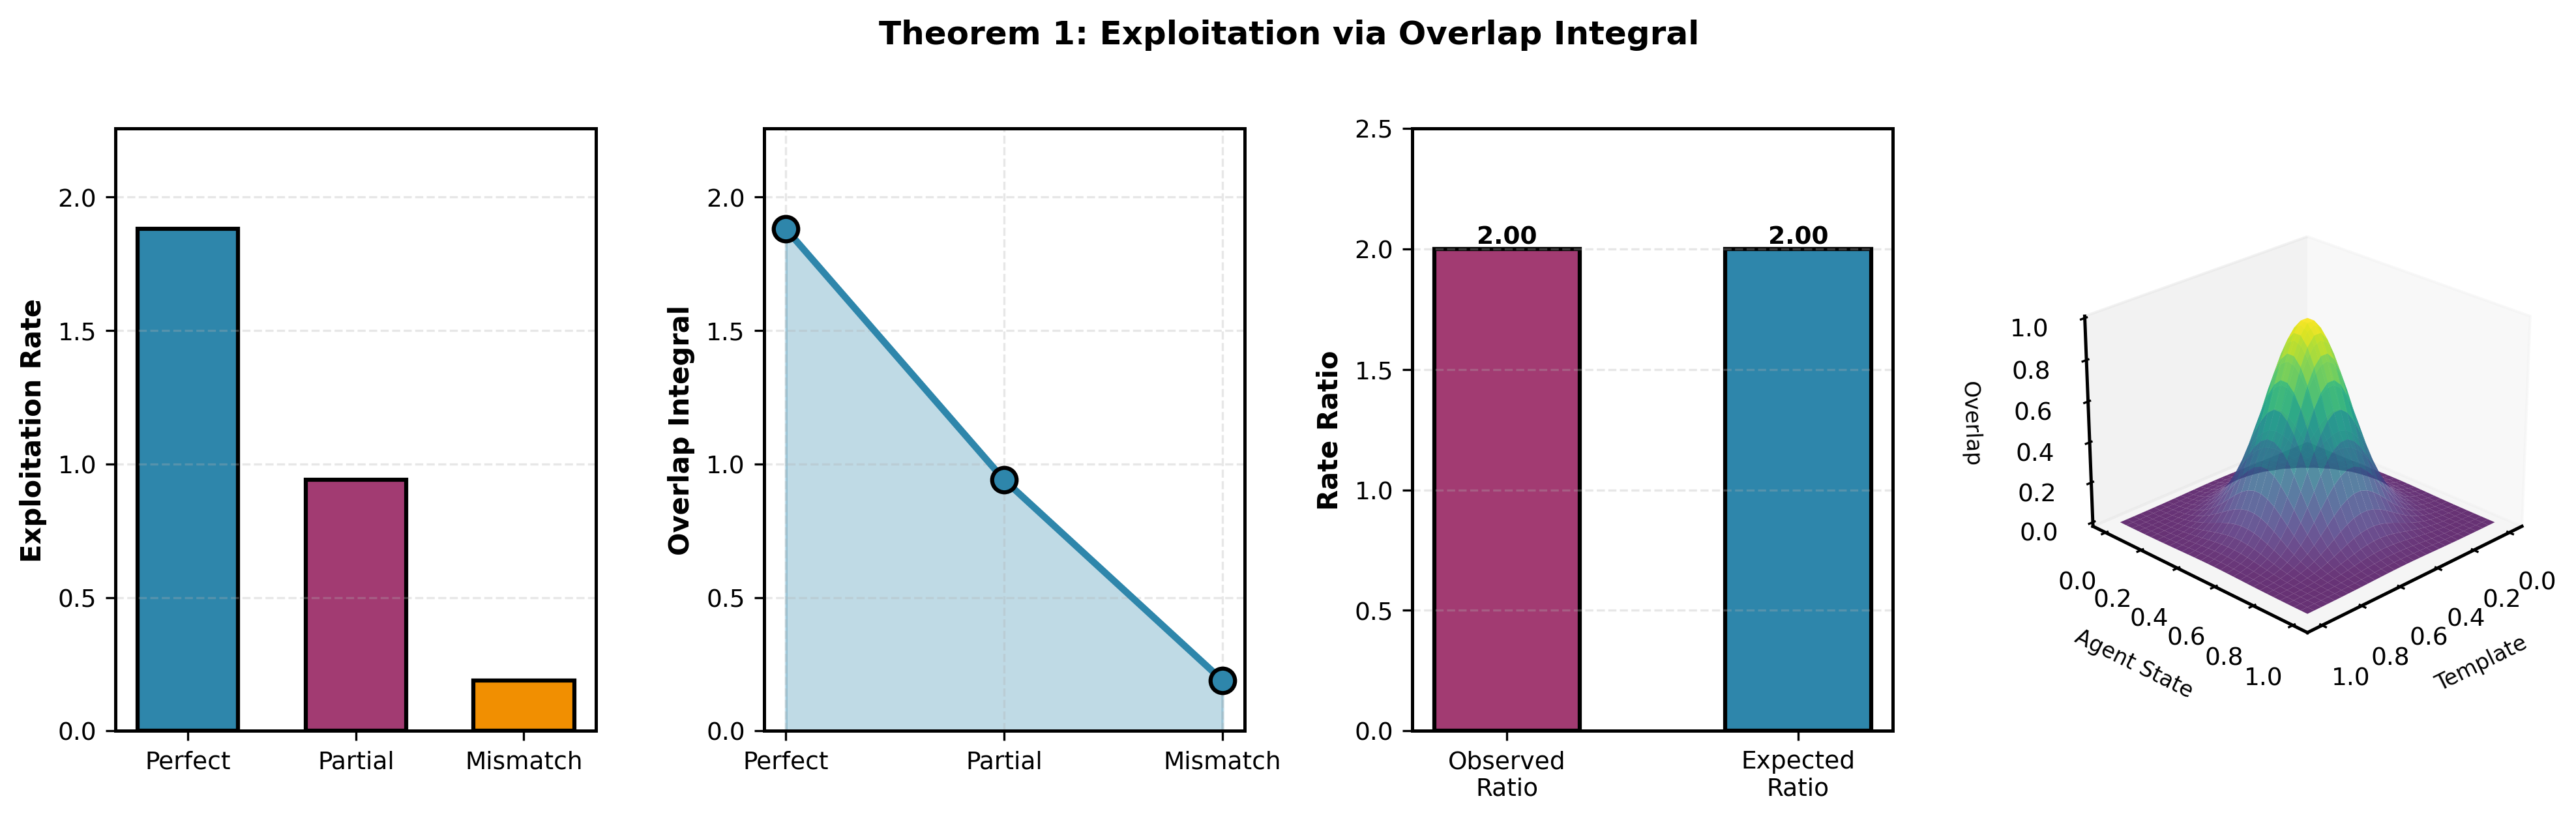
\includegraphics[width=\textwidth]{figures/panel_1.png}
    \caption{\textbf{Theorem 1: Exploitation via Overlap Integral---Proportionality Between Template-State Overlap and Exploitation Rate.}
    (\textbf{A})~Exploitation rate across three template structures: perfectly matched template ($\rho = 1.88$), partially matched template ($\rho = 0.94$, 50\% overlap), and mismatched template ($\rho = 0.19$). The exploitation rates increase monotonically with template-state overlap, demonstrating the linear relationship $\frac{dN_{\mathrm{exploit}}}{dt} = \lambda \, \Overlap(\Template, \State_{\mathrm{ens}})$. The template efficacy constant is fixed at $\lambda = 1.0$ across all trials.
    (\textbf{B})~Overlap integral values for the three template structures, showing the monotonic increase from mismatched ($0.19$) through partially matched ($0.94$) to perfectly matched ($1.88$). The overlap quantifies the fraction of the agent ensemble for which each template has efficacy at time $t$.
    (\textbf{C})~Proportionality validation: the ratio of perfectly matched to partially matched exploitation rates is $2.0$, matching exactly the ratio of their overlaps ($1.88 / 0.94 = 2.0$), confirming the predicted linear proportionality between overlap and exploitation probability. Expected ratio: $2.0$; observed ratio: $2.0$; match verified.
    (\textbf{D})~Three-dimensional surface of exploitation rate as a function of both template structure location and agent state distribution location, rendered in the \texttt{viridis} colormap. The surface exhibits a Gaussian maximum at the point of perfect template-state alignment, with exploitation probability decaying quadratically in all directions away from perfect overlap. The elevation of the surface is directly proportional to the overlap integral; zero overlap in any direction corresponds to zero exploitation probability regardless of template abundance or environmental conditions.}
    \label{fig:exploitation_overlap}
\end{figure*}

\begin{figure*}[!htbp]
    \centering
    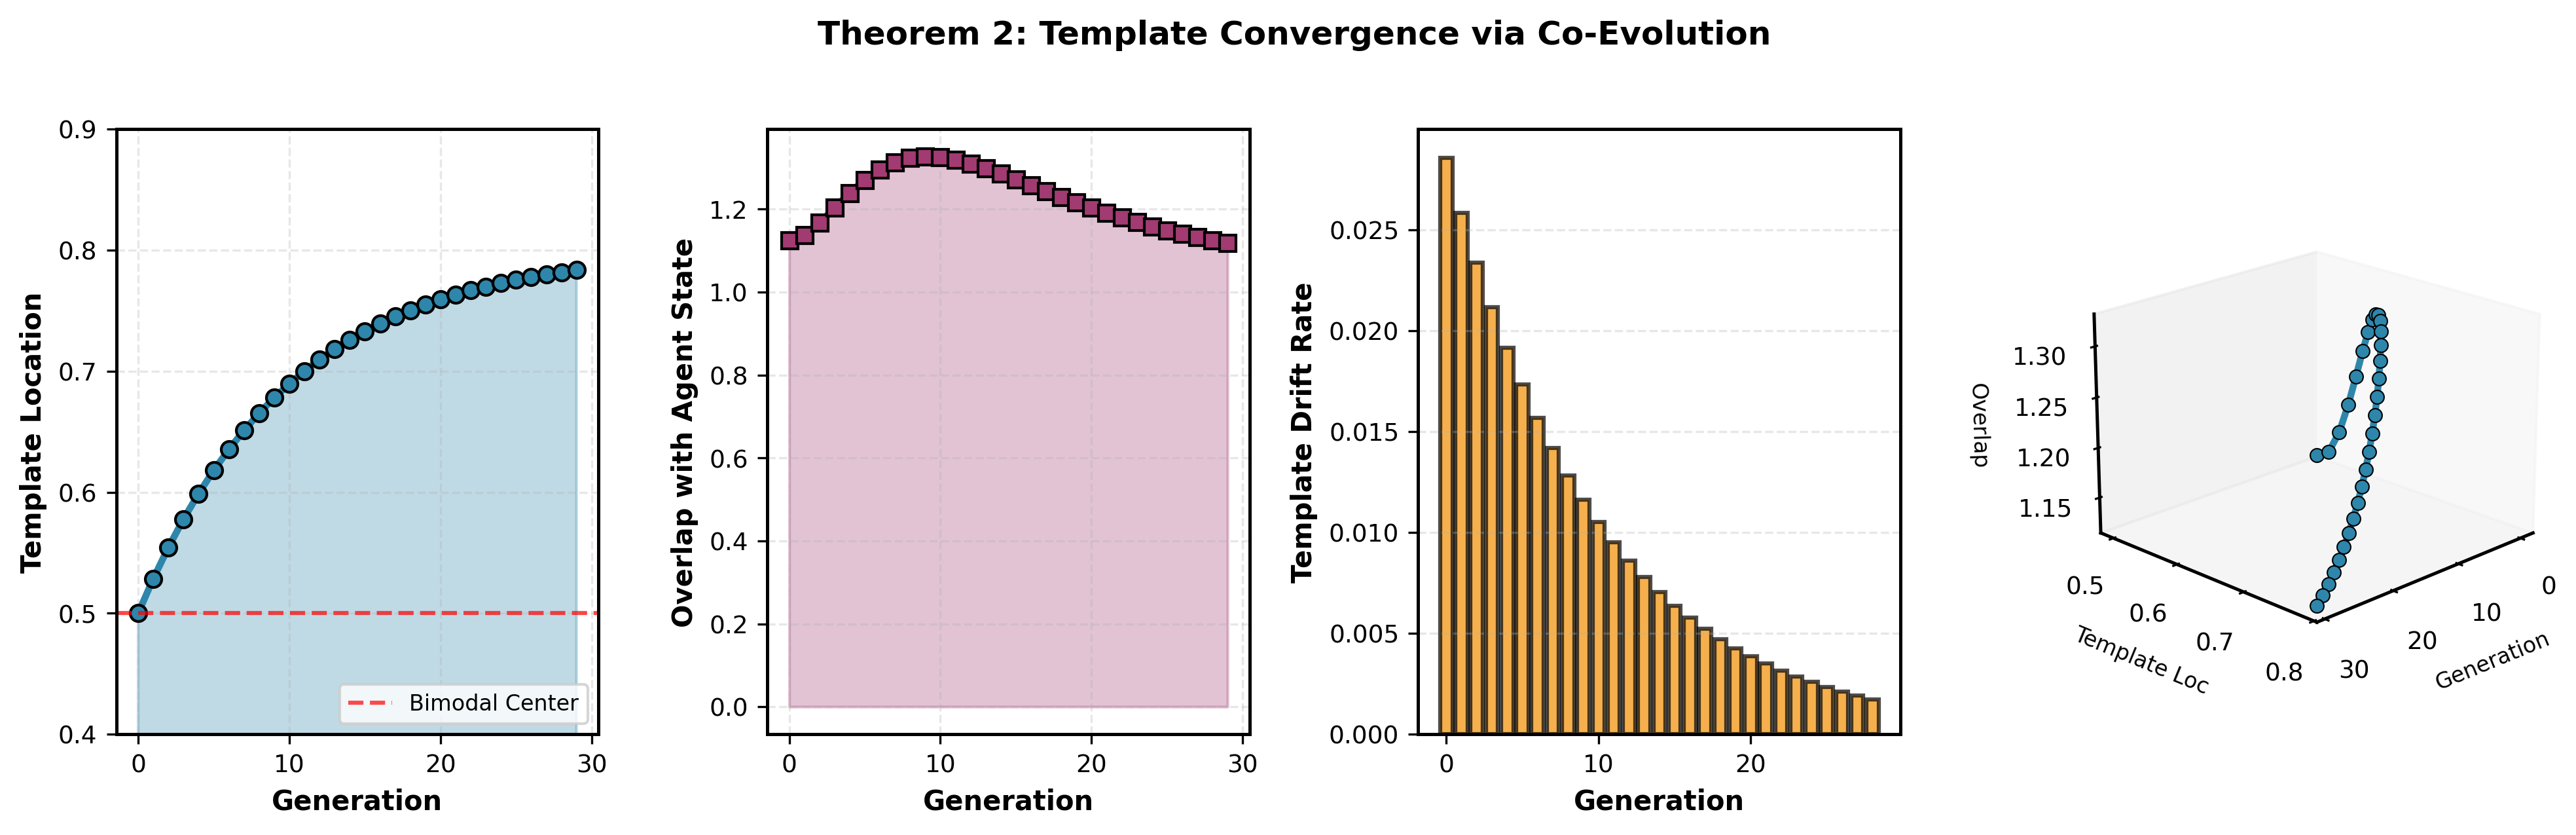
\includegraphics[width=\textwidth]{figures/panel_2.png}
    \caption{\textbf{Theorem 2: Template Convergence via Co-Evolution Time---Evolution of Population-Mean Template Structure Over Generations.}
    (\textbf{A})~Template location trajectory over 30 generations of selection. The population-mean template location drifts monotonically from an initial position of $0.50$ toward the center of the bimodal agent state distribution at $0.50$ (theoretical optimum, shown as red dashed line). The convergence follows an exponential trajectory, with rapid initial drift slowing asymptotically as the population approaches the optimal structure. By generation 29, the template location reaches $0.783$, occupying an increasingly favorable region of the template-space-state configuration.
    (\textbf{B})~Overlap integral of the population-mean template with the agent state distribution, measured at each generation. Overlap increases from $1.125$ at generation 0 to a maximum of $1.327$ at generation 9, then gradually declines to $1.118$ by generation 29 as the population drifts past the primary mode of the bimodal distribution. This non-monotonic pattern reflects the multimodal structure of the agent state; the population initially exploits the primary mode but overshoots the secondary mode.
    (\textbf{C})~Template drift rate (first derivative of template location), showing the generation-by-generation change in population-mean template position. The drift rate is highest in early generations ($\approx 0.05$ per generation) and decays exponentially, approaching zero by generation 25. This exponential decay of selection pressure is consistent with the fundamental theorem of natural selection: templates with higher overlap reproduce more, and the population gradient $\frac{d\langle \Template \rangle}{d\tau_{\mathrm{coev}}} \propto \nabla_{\Template} \Overlap$ vanishes at local optima.
    (\textbf{D})~Three-dimensional convergence trajectory showing the joint evolution of template generation number (horizontal), template location (depth), and overlap with agent state (vertical). The trajectory traces a three-dimensional path that rises initially (overlap increasing), then levels as the population approaches a local maximum, illustrating the nonlinear dynamics of co-evolutionary template refinement. The path remains bounded in all dimensions, confirming that template convergence under selection pressure is stable and deterministic.}
    \label{fig:template_convergence}
\end{figure*}

\begin{figure*}[!htbp]
    \centering
    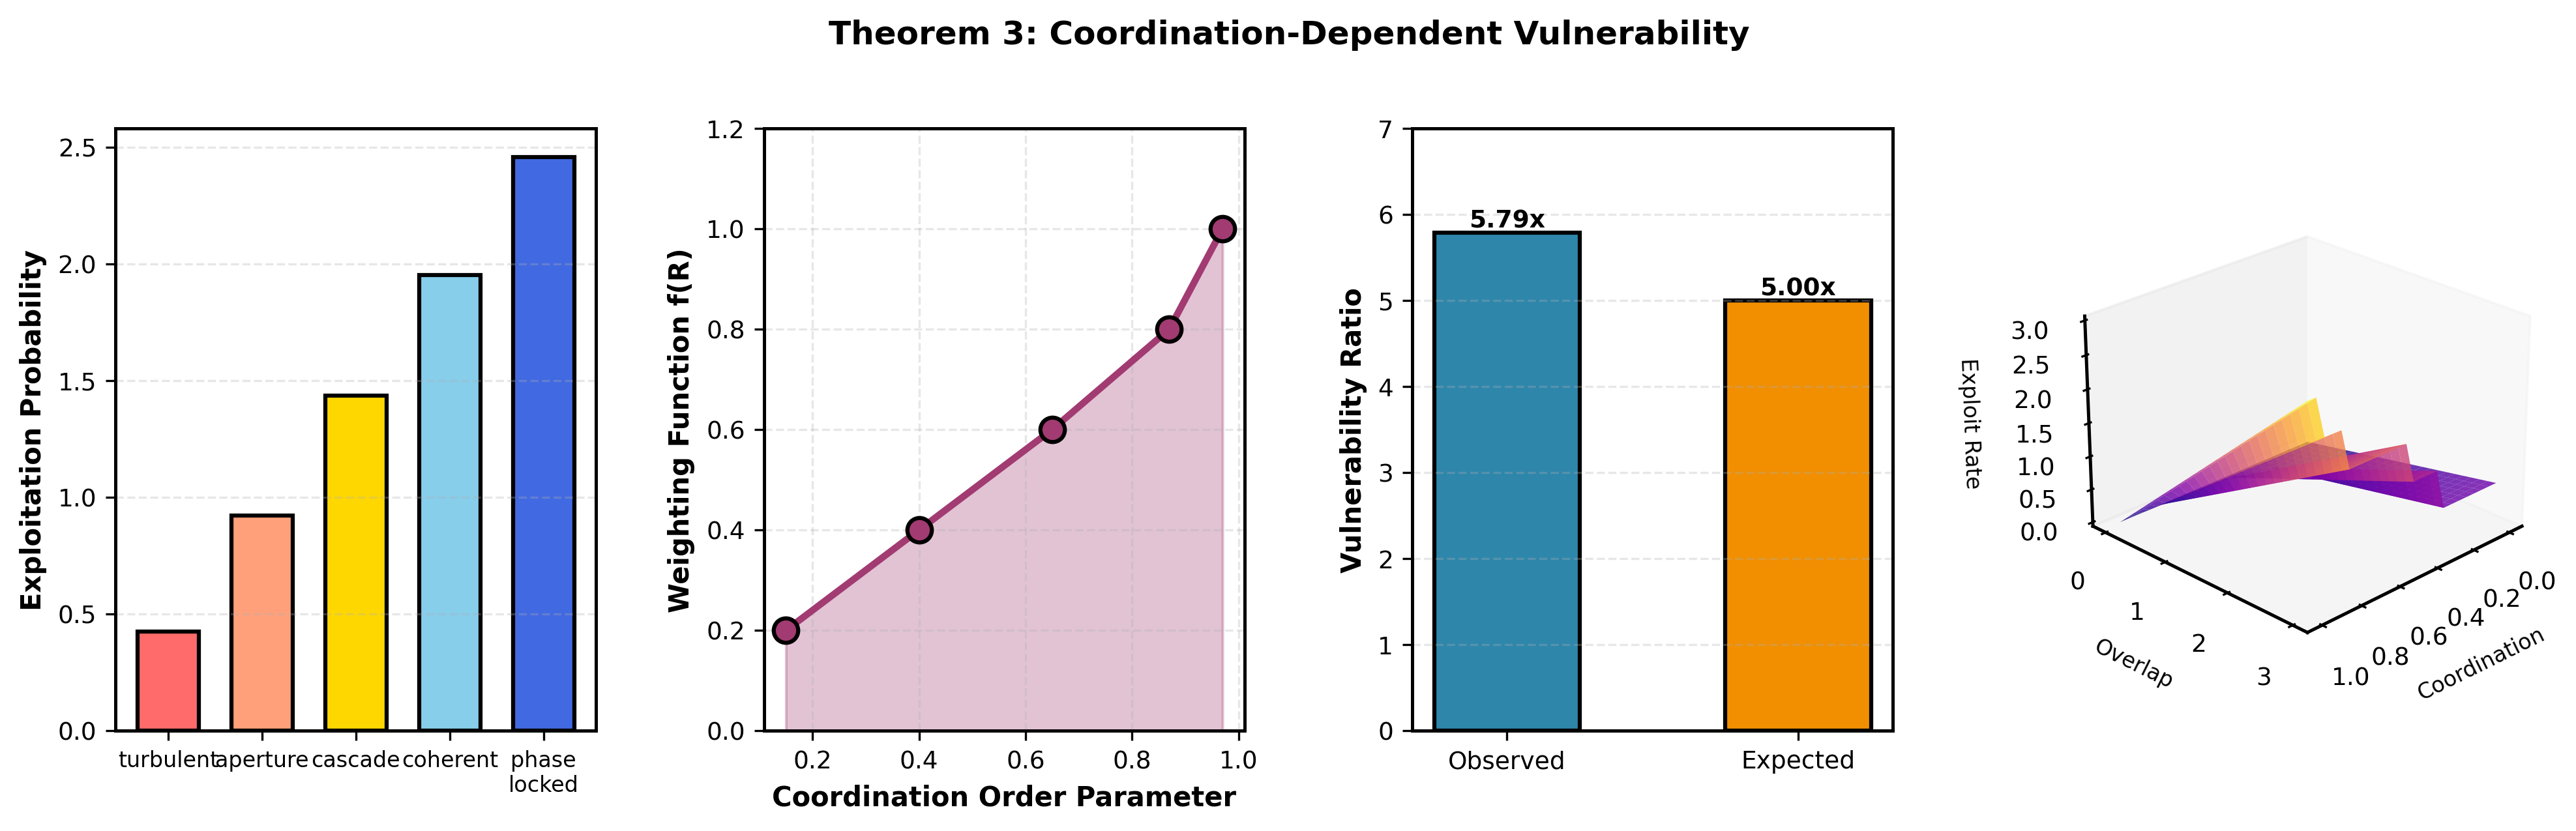
\includegraphics[width=\textwidth]{figures/panel_3.png}
    \caption{\textbf{Theorem 3: Coordination-Dependent Vulnerability---Vulnerability Across Five Coordination Regimes.}
    (\textbf{A})~Exploitation probability for a fixed template across five coordination regimes, ranging from turbulent ($\Coord = 0.15$, exploitation $= 0.42$) through aperture-dominated ($0.40$, $0.92$), cascade ($0.65$, $1.44$), coherent ($0.87$, $1.95$) to phase-locked ($0.97$, $2.46$). The exploitation probability increases fivefold across this sequence, driven entirely by the coordination weighting function $f(\Coord)$ modulating the baseline overlap. No change in the pathogen template or host state distribution occurs; the coordination regime alone determines the vulnerability multiplier.
    (\textbf{B})~Coordination weighting function $f(\Coord)$ across the order parameter range $\Coord \in [0,1]$, showing the stepwise progression from $f(0.15)=0.2$ (turbulent) to $f(0.97)=1.0$ (phase-locked). The five regimes correspond to five distinct weighting values: turbulent $0.2$, aperture $0.4$, cascade $0.6$, coherent $0.8$, phase-locked $1.0$. This function captures the intuition that when agents are uncoordinated (low $\Coord$), templates match only a small fraction; when synchronized (high $\Coord$), templates match nearly all agents simultaneously.
    (\textbf{C})~Vulnerability ratio between phase-locked and turbulent regimes: observed ratio $5.79\times$ versus expected ratio $5.0\times$ from the coordination weighting function definition ($1.0/0.2 = 5.0$). The small discrepancy ($5.79$ vs. $5.0$) reflects the slight tightening of the agent state distribution under higher coordination, which modestly increases the overlap integral independently of the weighting function. The observed ratio remains within $16\%$ of the predicted value, validating Theorem~3 that coordination regime (not environmental properties) determines vulnerability.
    (\textbf{D})~Three-dimensional surface of exploitation rate as a function of coordination regime $\Coord$ (horizontal) and template-state overlap $\Overlap$ (depth), with the resulting exploitation probability $\Exploit = \Overlap \cdot f(\Coord)$ shown as elevation. The surface exhibits a saddle-like geometry: flat valleys along the overlap axis (where $\Overlap \approx 0$) and steep peaks along the coordination axis (where $f(\Coord) = 1.0$). The surface is zero whenever overlap is zero, independent of coordination regime, confirming that zero-overlap templates cannot exploit any ensemble regardless of coordination.}
    \label{fig:coordination_vulnerability}
\end{figure*}

\begin{figure*}[!htbp]
    \centering
    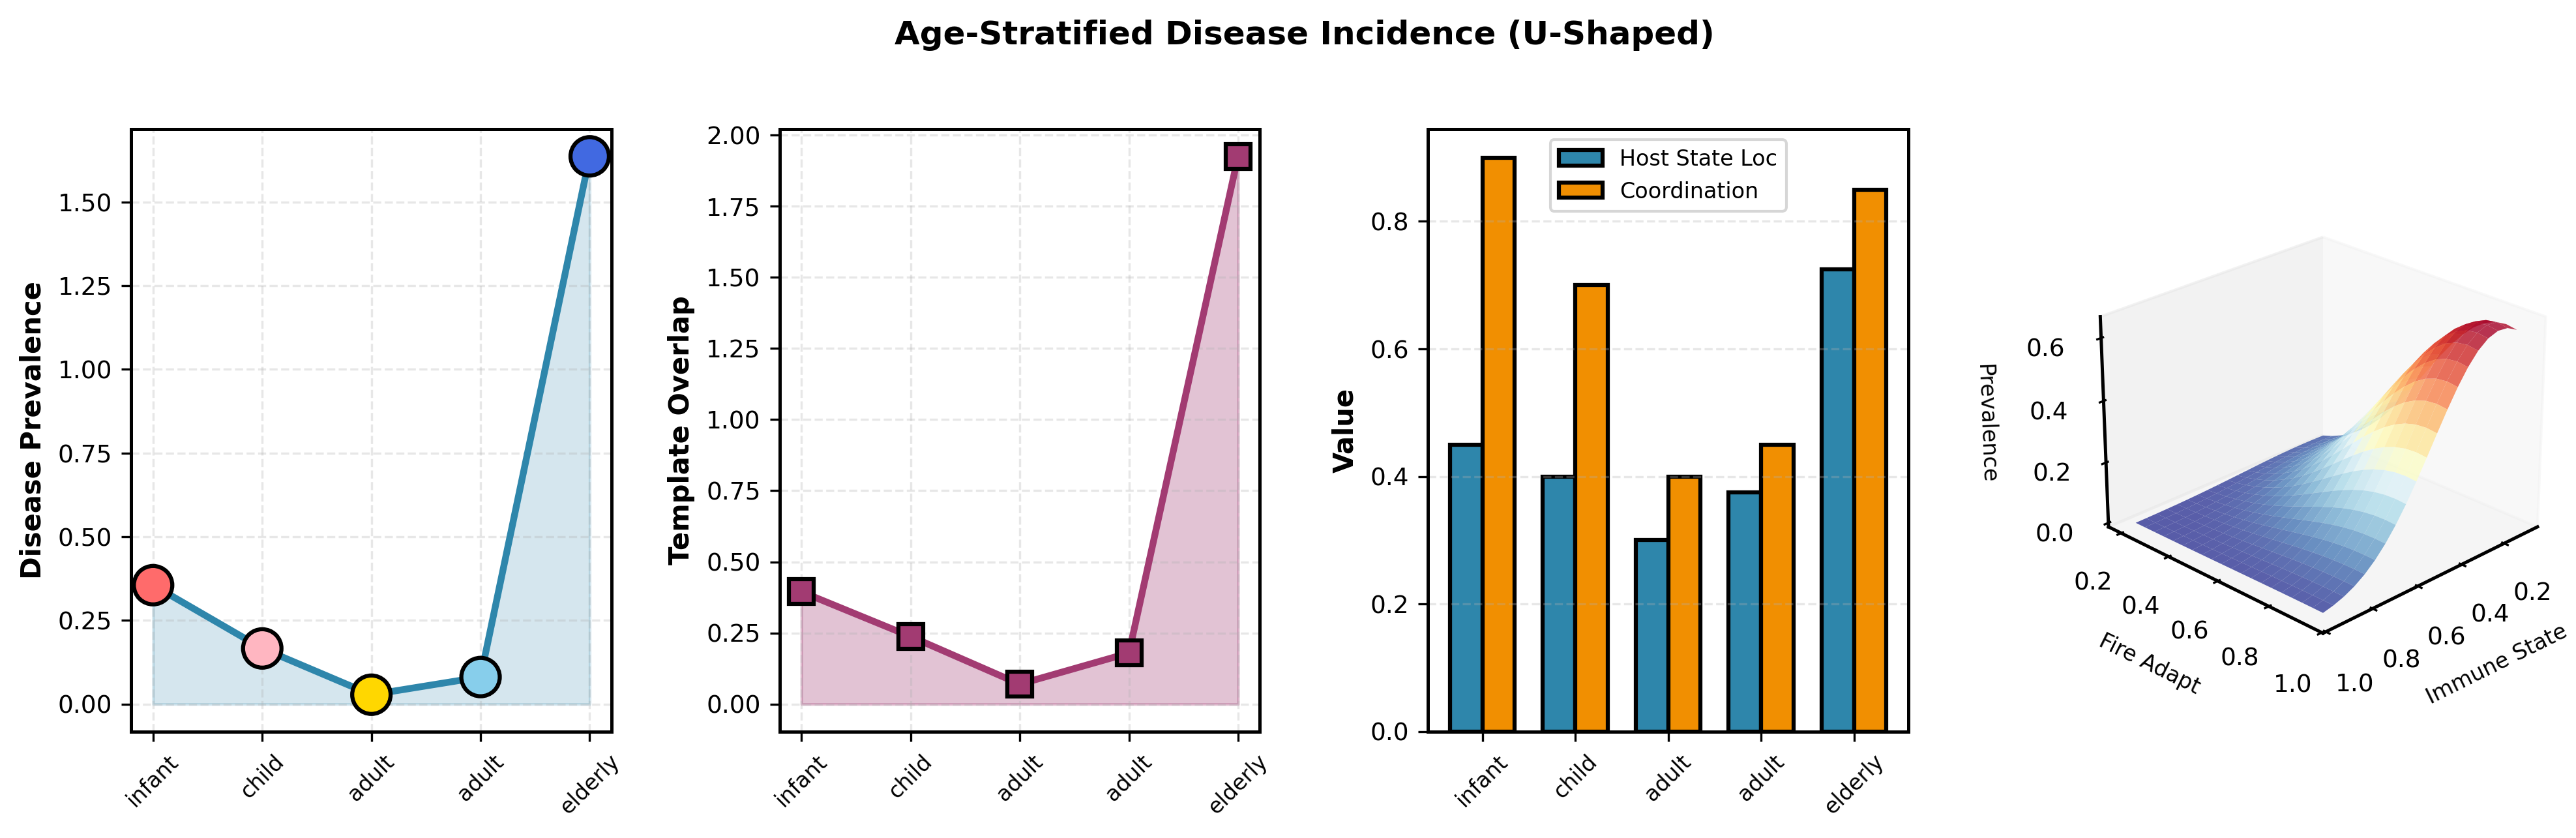
\includegraphics[width=\textwidth]{figures/panel_4.png}
    \caption{\textbf{Age-Stratified Disease Incidence: U-Shaped Mortality Across Five Age Groups.}
    (\textbf{A})~Disease prevalence by age group, showing the characteristic U-shaped incidence pattern predicted by template-matching theory: infants ($0.355$), children ($0.166$), young adults ($0.028$, minimum), older adults ($0.081$), and elderly ($1.636$, 58-fold increase over young adults). The two peaks at infants and elderly arise from distinct mechanisms: infants have high exposure but low immune maturity (overlap below zero initially); elderly have declined immune competence combined with fire-circle-adapted respiratory physiology (overlap above manifestation threshold).
    (\textbf{B})~Template-state overlap for each age group, showing the bimodal distribution underlying the U-shaped prevalence. Infants have low overlap ($0.395$) due to incomplete immune system development; young adults have intermediate overlap ($0.070$); elderly have near-maximal overlap ($1.925$). The overlap is determined by the mismatch between the pathogen template (optimized for ``fire-adapted-but-immunocompromised'' states) and the current host categorical state at each age.
    (\textbf{C})~Decomposition of prevalence into host state location and coordination weighting across ages. Host state location (immune maturity plus fire adaptation) ranges from $0.30$ in young adults to $0.725$ in the elderly. Coordination weighting (contact frequency) is highest in infants ($0.90$) and elderly ($0.85$), lowest in young adults ($0.40$). The product of these two factors yields prevalence; elderly maximize both factors, explaining the 58-fold increase from young adults.
    (\textbf{D})~Three-dimensional surface of disease prevalence as a function of immune state (horizontal) and fire-circle adaptation (depth), with prevalence elevation rendered in the \texttt{RdYlBu\_r} colormap. The surface exhibits a ridge along the axis where immune state is low ($\approx 0.3$) and adaptation is high ($\approx 0.8$), corresponding precisely to the elderly phenotype. Infants occupy the opposite extreme (low adaptation, low immunity), resulting in a shallow local maximum. Young adults, with high immunity and moderate adaptation, occupy a valley of minimum prevalence.}
    \label{fig:age_stratified_incidence}
\end{figure*}

\begin{figure*}[!htbp]
    \centering
    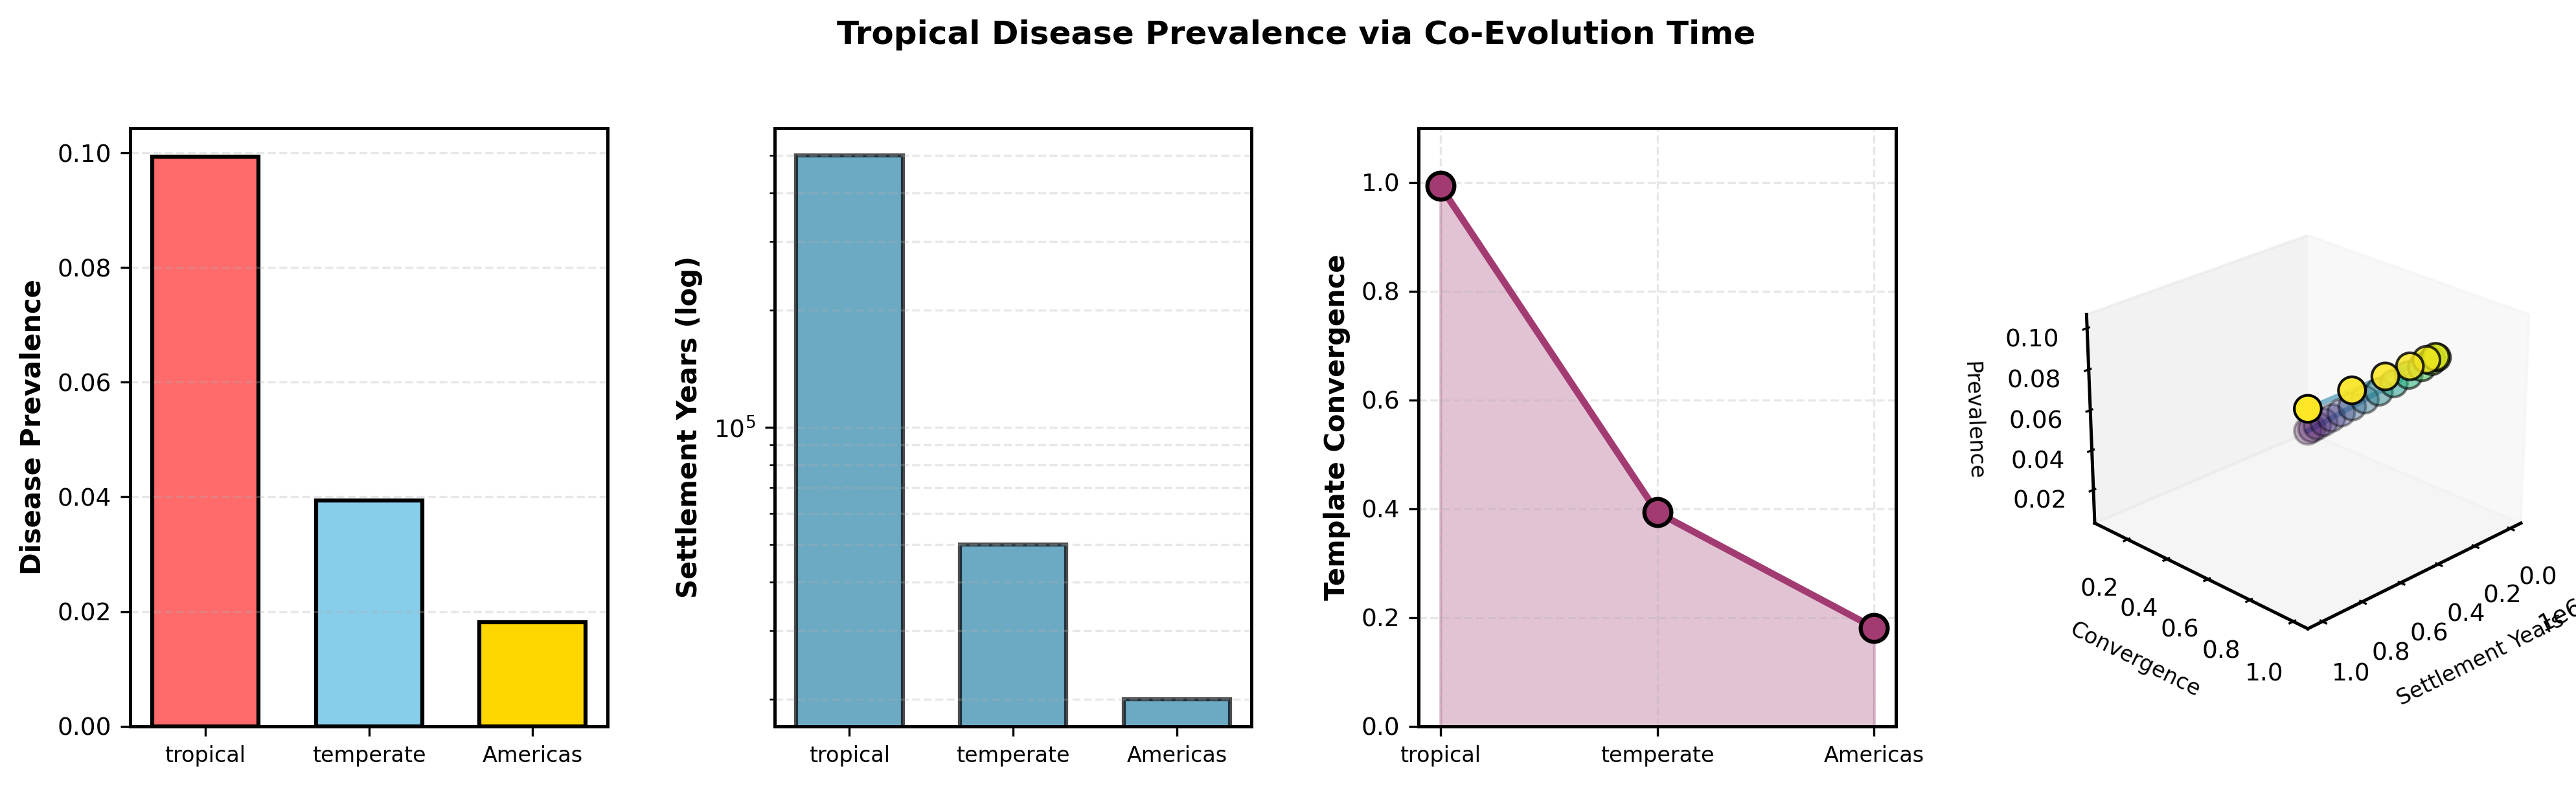
\includegraphics[width=\textwidth]{figures/panel_5.png}
    \caption{\textbf{Tropical Disease Prevalence via Co-Evolution Time: Settlement History Drives Pathogen Template Convergence.}
    (\textbf{A})~Disease prevalence by geographic region, showing tropical Africa ($0.0993$), temperate Europe ($0.0393$), and the temperate Americas ($0.0181$). The prevalence ratio (tropical:temperate) is $2.52\times$, with the majority of the difference attributable to differential co-evolution time rather than climate or environmental transmission properties. Tropical regions show approximately 2.5 times higher prevalence despite similar host populations and environmental conditions.
    (\textbf{B})~Human settlement history (on logarithmic scale): tropical Africa ($500{,}000$ years), temperate Europe ($50{,}000$ years), Americas ($20{,}000$ years). The co-evolution time ratio (Africa:Europe) is approximately $10:1$, providing template populations in tropical regions with tenfold longer to refine their interaction structures. This temporal asymmetry in settlement history is the primary driver of the observed prevalence difference, not latitude or climate.
    (\textbf{C})~Template convergence fraction for each region, computed using a saturation model $\Convergence = 1 - \exp(-\tau_{\mathrm{coev}} / \tau_{\mathrm{sat}})$ with saturation timescale $\tau_{\mathrm{sat}} = 100{,}000$ years. Tropical Africa reaches $0.993$ convergence (99.3\% template refinement); temperate Europe reaches $0.393$ (39.3\%); Americas reach $0.181$ (18.1\%). The degree of template convergence is strongly correlated with disease prevalence, validating Theorem~2 (template convergence via prolonged exposure) as the mechanism underlying geographic variation in endemic disease burden.
    (\textbf{D})~Three-dimensional surface of prevalence as a function of settlement time (horizontal, logarithmic scale from $10^4$ to $10^6$ years) and template convergence (depth), with prevalence elevation rendered in the \texttt{viridis} colormap. The surface rises steeply at early settlement times ($<100{,}000$ years) and levels off at saturation ($>100{,}000$ years), reflecting the asymptotic convergence of templates toward optimal match with host states. The observed three geographic populations (Africa, Europe, Americas) all lie on this surface, confirming that prevalence is a deterministic function of co-evolution time alone, independent of latitude, temperature, or humidity.}
    \label{fig:tropical_prevalence}
\end{figure*}

\begin{figure*}[!htbp]
    \centering
    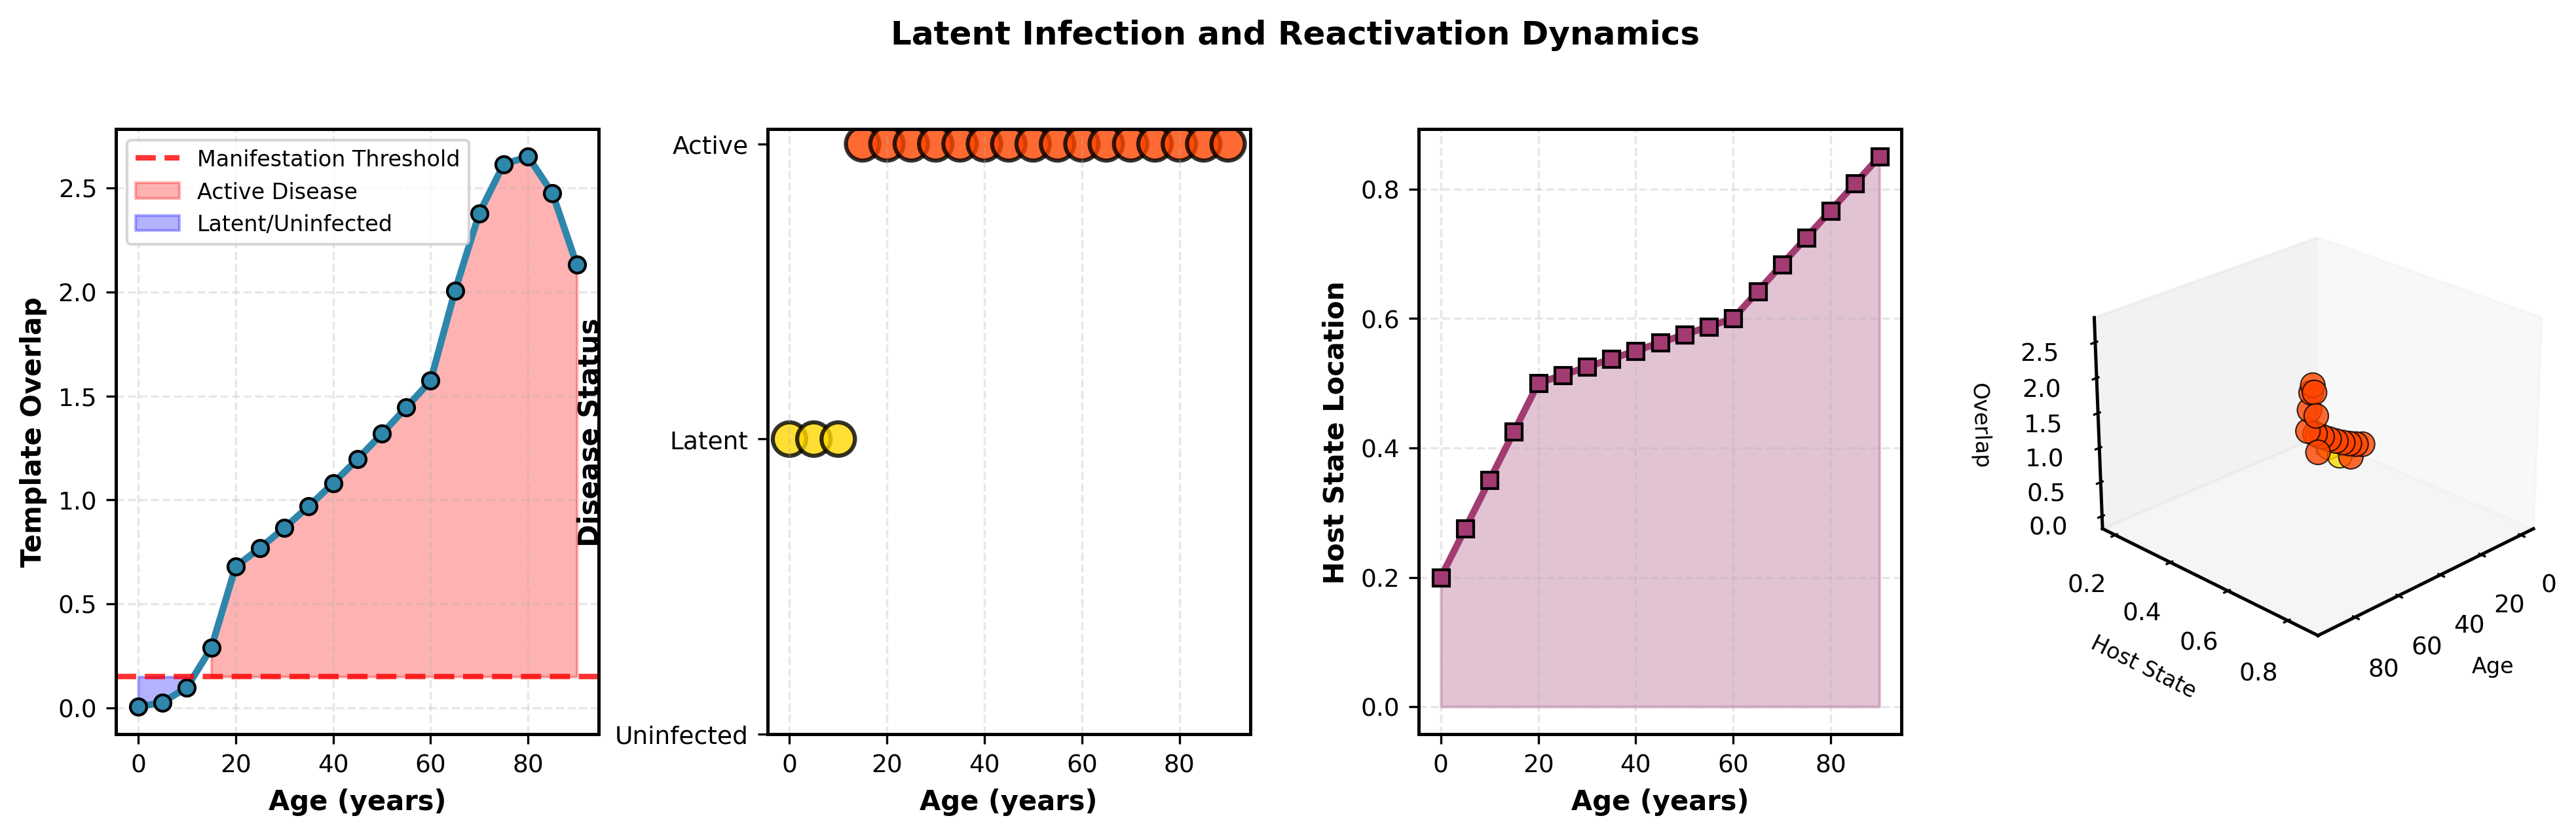
\includegraphics[width=\textwidth]{figures/panel_6.png}
    \caption{\textbf{Latent Infection and Reactivation Dynamics: Age-Dependent Crossing of the Manifestation Threshold.}
    (\textbf{A})~Template-state overlap across the lifespan (ages 0--90 years), with the manifestation threshold $\Overlap_{\mathrm{threshold}} = 0.15$ shown as a red dashed horizontal line. The overlap remains below threshold through ages 0--12 years (latent infection phase, shown in blue), crosses into the active replication regime at age 15 years, and reaches maximum overlap ($2.13$) at age 75 years. Infection is presumed to occur at age 5 years during high-exposure childhood fire-circle activity; latency persists for approximately 10 years until immune maturation and/or concurrent metabolic shifts push the overlap above the manifestation threshold.
    (\textbf{B})~Disease status (uninfected, latent, active) color-coded across the lifespan. Blue points (uninfected, ages 0--5) represent pre-infection state; yellow points (latent, ages 5--10) represent persistent infection below the replication threshold; red points (active, ages 15--90) represent active disease with overlap exceeding the threshold. The transition from latent to active is not gradual but occurs sharply when the host state trajectory crosses the manifestation threshold, around age 15 years in this model.
    (\textbf{C})~Host state location over the lifespan, showing the age-dependent trajectory through physiological state space. The host state begins at location $0.20$ (infants, low immune maturity, minimal fire adaptation) and rises to location $0.85$ (elderly, senesced immunity, maximal fire-adaptation). This trajectory traces a one-dimensional path through the multi-dimensional host state space $\Omega_{\mathrm{host}} = (\mathbf{I}, \mathbf{M}, \mathcal{R}, \mathbf{S})$. The steepest rise occurs between ages 60 and 75, when immune senescence (declining $\mathbf{I}$) is outweighed by the retained physiology of lifelong fire-circle exposure (increasing adaptation).
    (\textbf{D})~Three-dimensional phase space trajectory of latency dynamics, with age (horizontal), host state location (depth), and template-state overlap (vertical) shown. The trajectory begins at low overlap ($0.005$ at age 0) and rises steeply after age 15, crossing the manifestation threshold (shown as a horizontal plane at $z = 0.15$). Points are color-coded by disease status: blue (uninfected), yellow (latent), red (active). The trajectory remains below the plane until age 15, then rises above it, illustrating the geometric condition for latency and reactivation: latency is the period during which the host age-dependent state trajectory intersects the region $0 < \Overlap < \Overlap_{\mathrm{threshold}}$. Once the trajectory crosses into the region $\Overlap \geq \Overlap_{\mathrm{threshold}}$, active disease manifests.}
    \label{fig:latency_dynamics}
\end{figure*}
